\documentclass[11pt,a4paper]{article}

% --- Essential Packages ---
\usepackage[utf8]{inputenc}
\usepackage[margin=0.8in, top=0.85in, bottom=0.85in]{geometry}
\usepackage{titlesec}
\usepackage{hyperref}
\usepackage{graphicx}
\usepackage{booktabs}
\usepackage{tabularx}
\usepackage{enumitem}
\usepackage{fancyhdr}
\usepackage{tikz}
\usetikzlibrary{shapes.geometric, arrows, positioning, calc}
\usepackage{xcolor}
\usepackage{listings}
\usepackage{array}
\usepackage{tcolorbox}
\usepackage{float}

% --- Color Palette ---
\definecolor{primary}{RGB}{14, 116, 144}   % Deep Ocean Cyan
\definecolor{secondary}{RGB}{15, 23, 42}  % Slate Navy 900
\definecolor{accent}{RGB}{234, 88, 12}    % Deep Orange
\definecolor{lightgray}{RGB}{248, 250, 252}
\definecolor{boxgray}{RGB}{241, 245, 249}

% --- Hyperlink Setup ---
\hypersetup{
    colorlinks=true,
    linkcolor=primary,
    filecolor=primary,      
    urlcolor=primary,
    citecolor=primary,
    pdftitle={TravelUp Global - University Project Proposal},
    pdfpagemode=FullScreen,
}

% --- Header and Footer Styling ---
\pagestyle{fancy}
\fancyhf{}
\lhead{\textcolor{secondary}{\small\textbf{TravelUp Global} --- Course Project Proposal}}
\rhead{\textcolor{secondary}{\small Markup \& Scripting Languages Lab}}
\cfoot{\small\thepage}
\renewcommand{\headrulewidth}{0.5pt}

% --- Section Heading Formatting ---
\titleformat{\section}
  {\normalfont\large\bfseries\color{primary}}{\thesection}{0.8em}{}[\titlerule]
\titleformat{\subsection}
  {\normalfont\normalsize\bfseries\color{secondary}}{\thesubsection}{0.6em}{}
\titleformat{\subsubsection}
  {\normalfont\small\bfseries\color{accent}}{\thesubsubsection}{0.5em}{}

\titlespacing*{\section}{0pt}{10pt}{5pt}
\titlespacing*{\subsection}{0pt}{7pt}{3pt}
\titlespacing*{\subsubsection}{0pt}{5pt}{2pt}

% --- Compact Lists ---
\setlist{itemsep=1.5pt, topsep=2pt, parsep=0pt, partopsep=0pt}

% --- Code Listing Setup ---
\lstset{
  basicstyle=\ttfamily\scriptsize,
  breaklines=true,
  backgroundcolor=\color{lightgray},
  frame=single,
  rulecolor=\color{gray!30}
}

\begin{document}

% ==============================================================================
% PAGE 1: TITLE & COVER PAGE
% ==============================================================================
\begin{titlepage}
    \centering
    \vspace*{0.3cm}
    
    {\large\bfseries\textcolor{primary}{UNIVERSITY PROJECT PROPOSAL}}\\[0.2cm]
    {\color{primary}\rule{0.6\textwidth}{2.2pt}}\\[0.6cm]
    
    {\Huge \textbf{\textcolor{secondary}{TRAVELUP GLOBAL}}}\\[0.3cm]
    {\large \textbf{An Enterprise Dual-Portal Global Tourism and Dynamic Itinerary Engineering Platform}}\\[0.2cm]
    {\normalsize \textbf{Addressing Real-World Travel Complexities Beyond Social Media Limitations}}\\[0.55cm]
    
    % --- Metadata Specification Table ---
    \renewcommand{\arraystretch}{1.22}
    \begin{tabularx}{\textwidth}{@{}>{\bfseries}p{5.2cm} X@{}}
        Project Title           & TRAVELUP GLOBAL \\
        Project Type            & Full-Stack Web Application (Dual-Portal Architecture) \\
        Project Domain          & Dynamic Itinerary Engineering, Booking Logistics \& Fintech \\
        Submitted To            & Sajib Bhattacharjee \\
        Designation             & Lecturer \\
        Department              & Department of Computer Science \& Engineering (CSE) \\
        Institution             & Dhaka International University (DIU) \\
        Course Title            & Markup \& Scripting Languages Lab \\
        Submission Date         & 14/10/2026 \\
    \end{tabularx}
    
    \vspace{0.6cm}
    
    % --- Project Team Block ---
    {\bfseries\textcolor{secondary}{\large PROJECT TEAM}}\\[0.15cm]
    \renewcommand{\arraystretch}{1.25}
    \begin{tabularx}{\textwidth}{c X r}
        \toprule
        \textbf{No.} & \textbf{Student Name} & \textbf{Roll/ID} \\
        \midrule
        1 & Md. Tanvir Parvaj & 39 \\
        2 & Md. Toufick Hasan & 34 \\
        3 & Fahima Suborna    & 36 \\
        \bottomrule
    \end{tabularx}
    
    \vfill
    \begin{tcolorbox}[colback=boxgray,colframe=primary,arc=2mm,boxrule=0.8pt]
    \centering\footnotesize\textcolor{secondary}{
    \textbf{Core Academic Problem Statement Addressed in this Proposal:}\\
    \textit{``Why must modern travel logistics be implemented as an engineered Full-Stack Web Platform instead of a basic social media (Facebook) page or static marketing catalog?''}
    }
    \end{tcolorbox}
    \vspace*{0.1cm}
\end{titlepage}

\newpage

% ==============================================================================
% SECTION 1: EXECUTIVE ABSTRACT & PROBLEM STATEMENT
% ==============================================================================
\section{Executive Abstract \& Core Motivation}

\subsection{1.1 Abstract}
\textbf{TravelUp Global} (\texttt{travelupglobal.com}) is an integrated, full-stack, dual-portal travel discovery, dynamic itinerary engineering, and operational management platform. Developed in strict compliance with the \textbf{Markup \& Scripting Languages Lab} curriculum, the system unifies semantic HTML5 document structures, hardware-accelerated CSS3 layout models, event-driven reactive client scripting (Vanilla ES6+), asynchronous RESTful microservices (Node.js/Express), and a relational Hostinger MySQL database engine with 3NF ACID compliance.

While traditional tourism businesses operate through static brochures or manual Facebook pages, modern tourism logistics requires dynamic multi-variable computation: resolving multi-leg intermodal transit, enforcing wheelchair accessibility constraints, executing automated meteorological refund webhooks, providing real-time split-bill group checkouts, and enforcing a six-tier Role-Based Access Control (RBAC) security matrix. TravelUp Global replaces chaotic manual communication with deterministic software architecture.

\subsection{1.2 Problem Statement: The Digital Logistics Void}
\begin{itemize}[leftmargin=*]
    \item \textbf{Manual Communication Latency:} Booking travel via social media channels requires hours of back-and-forth messaging, manual quotation errors, and high rate of booking friction.
    \item \textbf{Rigid Monolithic Packaging:} Commercial tour providers enforce rigid, pre-packaged bundles without giving travelers the freedom to skip transport, choose distinct individual activities, or select specialized bedding.
    \item \textbf{Zero Real-Time Concurrency \& Double-Booking Risks:} Manual record-keeping in spreadsheets or social media direct messages lacks database transactional isolation (ACID), leading to disastrous overbooking incidents.
    \item \textbf{Financial Opacity \& Payment Disasters:} Group tours currently rely on a single traveler fronting costs via personal mobile money (bKash), leading to unverified transaction disputes, lack of fiscal receipts, and zero corporate VAT accounting.
\end{itemize}

% ==============================================================================
% SECTION 2: ACADEMIC DEFENSE: WEB PLATFORM VS. FACEBOOK PAGE
% ==============================================================================
\section{Architectural Defense: Full-Stack Web Application vs. Facebook Page}

A central question in software evaluation is: \textit{``Can this system be replaced simply by creating a Facebook page and chatting on Messenger?''} From a software engineering perspective, social media pages are merely presentation boards for unstructured text and images. They lack database persistence, reactive algorithmic computation, cryptographic security, and transaction atomicity. Table~\ref{tab:fb_vs_web} provides a definitive technical comparison.

\begin{table}[H]
\centering
\scriptsize
\renewcommand{\arraystretch}{1.2}
\begin{tabularx}{\textwidth}{p{2.6cm} p{5.0cm} X}
\toprule
\textbf{Functional Dimension} & \textbf{Social Media (Facebook Page / Messenger)} & \textbf{TravelUp Global Full-Stack Engineering Platform} \\
\midrule
\textbf{Inventory \& Concurrency} & Static photo posts; zero relational state. Double-bookings occur frequently due to uncoordinated human chat agents. & Hostinger MySQL relational 3NF schema with ACID transactions, atomic row locks, and real-time inventory decrementing. \\
\addlinespace
\textbf{Pricing \& Route Calculation} & Manual quote guessing by admins. Cannot dynamically compute multi-leg flight + microbus routes with transfer buffers. & Client-side reactive JavaScript DOM + REST API synthesizing intermodal transit routes and live itemized price breakdowns. \\
\addlinespace
\textbf{Customization \& Bedding Logic} & Fixed ``take-it-or-leave-it'' packages. Inquiries about 4-bed family rooms or skipping transport require manual quote recalculation. & Modular Custom Trip Builder with \texttt{[✓] Skip Transport} toggles, bed configuration formulas, and individualized per-person pricing. \\
\addlinespace
\textbf{Group Split-Billing (Fintech)} & Single student must collect cash or receive 30 unverified bKash personal transfers with severe ledger confusion. & Automated \textit{Shareable Split-Bill Payment Link} generating unique transaction tokens and real-time live paid status indicator ticks. \\
\addlinespace
\textbf{Medical \& Physical Constraints} & Human chat admins overlook elderly wheelchair needs or seafood allergies, booking inaccessible hilltop cottages. & Multi-faceted relational filtering algorithmically pruning properties lacking elevator/wheelchair access or non-allergic menus. \\
\addlinespace
\textbf{Automated Weather Refunds} & Manual disputes over days or weeks when coastal storms halt sea tours; money held indefinitely. & Meteorological alert triggers instantly broadcast warning severity, halt hazardous tours, and execute auto-refunds to user wallets. \\
\addlinespace
\textbf{Corporate Compliance \& B2B} & Cannot generate legally compliant NBR VAT/Tax challans, corporate purchase orders, or auditor ledgers. & Automated B2B quotation engine calculating corporate tax tiers, producing printable PDF invoices with fiscal breakdown. \\
\addlinespace
\textbf{Cryptographic Security \& RBAC} & All staff share page login credentials; interns possess identical privileges to owners; zero audit logs. & Cryptographic JWT authorization with 6-Tier Enterprise RBAC strictly isolating Superadmin, Manager, Accountant, and Support. \\
\bottomrule
\end{tabularx}
\caption{Technical Justification: Facebook Page Limitations vs. TravelUp Global Engineering Architecture}
\label{tab:fb_vs_web}
\end{table}

\newpage

% ==============================================================================
% SECTION 3: ENGINEERING VERIFICATION: 12 REAL-WORLD SCENARIOS
% ==============================================================================
\section{Engineering Verification: 12 Real-World Complex Travel Scenarios}

To substantiate that TravelUp Global is an essential computational engine rather than a static catalog, this section presents twelve rigorous, real-world travel scenarios mapped directly to our platform's algorithms.

\subsection{Category A: Intermodal Transit \& Dynamic Routing Engine}

\subsubsection{Scenario 1: Multi-Leg Route Synthesis (Panchagarh-Tetulia via Syedpur)}
\begin{itemize}[leftmargin=*]
    \item \textbf{Traveler Persona:} Tanzim (Freelance Landscape Photographer traveling from Dhaka to capture Kanchenjunga).
    \item \textbf{Logistical Barrier:} Tetulia possesses no regional airport. Manual inquiry requires independently booking an airline ticket, guessing landing times, and haggling with ground microbus drivers at Syedpur.
    \item \textbf{TravelUp Algorithmic Solution:} The platform's Intermodal Route Resolver programmatically pairs Leg 1 (\texttt{DAC} $\rightarrow$ \texttt{SPD} Flight: \textdied4,500) with Leg 2 (\texttt{SPD} $\rightarrow$ Tetulia connecting shared AC microbus: \textdied800), factoring in a 45-minute baggage transfer buffer. Tanzim secures a unified joint e-ticket in a single checkout.
\end{itemize}

\subsubsection{Scenario 2: Open-Ended Telecommuting Stay with Dynamic Return Seat Allocation}
\begin{itemize}[leftmargin=*]
    \item \textbf{Traveler Persona:} Farhan (Remote Software Developer relocating to Sajek Valley for co-working).
    \item \textbf{Logistical Barrier:} Farhan does not know whether his sprint requires 3 days or 7 days; fixed return tickets waste capital, while social media tour operators refuse open-ended stays.
    \item \textbf{TravelUp Algorithmic Solution:} Farhan selects one-way transit with 3 initial cottage nights. The booking is flagged with \texttt{Open-Return Status}. When ready to return, his dashboard queries live unallocated seats on returning agency buses or integrates him into returning tour cohorts at discounted rates.
\end{itemize}

\subsubsection{Scenario 3: Runtime Seat Layout \& Dynamic Counter Contact Telematics}
\begin{itemize}[leftmargin=*]
    \item \textbf{Traveler Persona:} Sadia \& Friend (Female university students departing Arambagh counter at 11:30 PM).
    \item \textbf{Logistical Barrier:} Fear of rear bus turbulence, desire for forward female-safe seating, and anxiety regarding midnight counter coordination.
    \item \textbf{TravelUp Algorithmic Solution:} The client interface renders an SVG bus seat matrix enforcing female-preference forward row allocation. Upon booking confirmation, the dynamic voucher generator extracts real-time database records to print the active mobile numbers of both the Arambagh Counter Manager and the Bus Supervisor.
\end{itemize}

\subsubsection{Scenario 4: Decoupled 'No-Transport' Self-Drive Trip Builder}
\begin{itemize}[leftmargin=*]
    \item \textbf{Traveler Persona:} Asif \& 4 Friends (Private SUV road-trip enthusiasts driving their own Toyota Prado to Sylhet).
    \item \textbf{Logistical Barrier:} Conventional agencies demand payment for monolithic packages including unwanted bus fares.
    \item \textbf{TravelUp Algorithmic Solution:} The Custom Trip Builder includes a reactive \texttt{[✓] Skip Transport} state toggle. The calculation engine subtracts transit fares while seamlessly provisioning 4 resort rooms, Jaflong registered motorized boat permits, and certified local guides.
\end{itemize}

\subsection{Category B: Accommodation, Bedding \& Accessibility Constraints}

\subsubsection{Scenario 5: Multi-Bed Room Allocation \& Per-Person Cost Optimization}
\begin{itemize}[leftmargin=*]
    \item \textbf{Traveler Persona:} Rahat \& 3 University Friends (Budget-conscious travelers visiting Cox's Bazar).
    \item \textbf{Logistical Barrier:} Booking two separate twin rooms doubles lodging expenses beyond student budgets.
    \item \textbf{TravelUp Algorithmic Solution:} The hotel inventory database models detailed bedding types: \textit{``Deluxe 4-Bed Family Room (2 King Beds)''} at \textdied3,500/night. The reactive calculation engine decomposes the total price down to \textdied875/person/night, updating the dynamic student cost summary in real time.
\end{itemize}

\subsubsection{Scenario 6: Strict Accessibility \& Medical Ground Constraints}
\begin{itemize}[leftmargin=*]
    \item \textbf{Traveler Persona:} Jamil (Banker traveling with his 70-year-old mother who has severe arthritis and a diabetic father).
    \item \textbf{Logistical Barrier:} Hilltop cottages with steep, unpaved outdoor stairs are physically hazardous.
    \item \textbf{TravelUp Algorithmic Solution:} The traveler applies the \texttt{[✓] Wheelchair \& Elevator Accessible} filter. The SQL query executes \texttt{WHERE has\_elevator = 1 AND ground\_floor\_available = 1}, immediately pruning inaccessible properties and recommending level-ground resorts with roll-in facilities.
\end{itemize}

\subsubsection{Scenario 7: Modular Micro-Addons \& Early Morning Fresh-up Calculation}
\begin{itemize}[leftmargin=*]
    \item \textbf{Traveler Persona:} Touhid \& Riya (Honeymoon couple) / Mahin (Executive arriving Sreemangal at 5:30 AM).
    \item \textbf{Logistical Barrier:} Standard hotel check-in is strictly 12:00 PM; travelers must either wait 6 hours on the street or purchase an entire extra day. Honeymoon decor requests are often forgotten in chat messages.
    \item \textbf{TravelUp Algorithmic Solution:} Checkbox add-ons dynamically append \textit{``Honeymoon Flower Bed Decoration (+1,500)''} and \textit{``Early Check-in Fresh-up Room (+35\% half-day rate)''}, updating the relational ledger without human intervention.
\end{itemize}

\subsection{Category C: Group Fintech, Dynamic Activity Splitting \& Safety Automation}

\subsubsection{Scenario 8: Disaggregated Group Activity Selection (Zero Forced Bundling)}
\begin{itemize}[leftmargin=*]
    \item \textbf{Traveler Persona:} 4-Friend Group at Inani Beach, Cox's Bazar.
    \item \textbf{Logistical Barrier:} 2 friends demand parasailing and speedboat thrill rides (\textdied2,300/person), while 2 friends prefer beachside coconut lounge relaxation (\textdied100). Social media operators force identical costs on everyone.
    \item \textbf{TravelUp Algorithmic Solution:} Our system features an individualized activity matrix where each sub-traveler's preferences are toggled separately and compiled into a single consolidated master reservation with itemized accountability.
\end{itemize}

\subsubsection{Scenario 9: Automated Meteorological Cancellation \& Instant Digital Wallet Refund}
\begin{itemize}[leftmargin=*]
    \item \textbf{Traveler Persona:} Sujan (Saint Martin traveler who prepaid \textdied3,000 for guided scuba diving).
    \item \textbf{Logistical Barrier:} Sudden Maritime Cautionary Signal No. 3 causes the Bangladesh Coast Guard to shut down diving. Manual refund processing through social media takes weeks of disputes.
    \item \textbf{TravelUp Algorithmic Solution:} The administrative alerts module broadcasts an active storm warning. The system evaluates all pending dive reservations for the affected timestamp, executes programmatic cancellation, and instantly credits \textdied3,000 back to the traveler's digital wallet/bKash account.
\end{itemize}

\subsubsection{Scenario 10: Granular Child Bedding \& Age-Tiered Fare Engine}
\begin{itemize}[leftmargin=*]
    \item \textbf{Traveler Persona:} Anis \& Family (Parents traveling with an infant of 3 years and a child of 7 years).
    \item \textbf{Logistical Barrier:} Calculating differential transit seats and hotel extra bedding manually leads to arithmetic errors.
    \item \textbf{TravelUp Algorithmic Solution:} Deterministic age-tier algorithm: Infant ($<4$ yrs) transit = \textdied0 (lap seat); Child ($5-10$ yrs) transit = \textdied800 (dedicated seat); Child with parents in existing bed = \textdied0 lodging; Optional rollaway extra mattress = \textdied500/night.
\end{itemize}

\subsubsection{Scenario 11: Corporate B2B Automated Quotation \& Official VAT/Tax Invoicing}
\begin{itemize}[leftmargin=*]
    \item \textbf{Traveler Persona:} Tanvir (HR Manager organizing a 25-employee tech company annual retreat in Sreemangal).
    \item \textbf{Logistical Barrier:} Corporate accounts require dedicated 30-seat AC bus chartering, 12 twin-bed rooms, conference hall reservations, and official NBR VAT/Tax compliance receipts for corporate tax filing.
    \item \textbf{TravelUp Algorithmic Solution:} The platform generates a B2B Corporate Group Quotation calculating volume tiered discounts, appending standard 15\% VAT and 5\% AIT, and outputting an audit-ready PDF invoice.
\end{itemize}

\subsubsection{Scenario 12: Batch Tour Collaborative Split-Payment Webhook (Split-Bill)}
\begin{itemize}[leftmargin=*]
    \item \textbf{Traveler Persona:} 30-Student University CSE Batch Tour (Total Itinerary Budget: \textdied1,50,000).
    \item \textbf{Logistical Barrier:} The student Class Representative cannot pay \textdied1,50,000 upfront. Manual collection via personal bKash leads to mismatched TrxIDs, caps, and disputes.
    \item \textbf{TravelUp Algorithmic Solution:} The checkout engine generates an authenticated \textit{Shareable Split-Bill Payment Link}. Each student accesses the portal, pays their exact \textdied5,000 share via bKash/Nagad/Cards, and the master reservation dashboard displays live real-time green ticks until 100\% quorum is reached.
\end{itemize}

\begin{tcolorbox}[colback=lightgray,colframe=secondary,arc=1mm,boxrule=0.6pt]
\footnotesize\textbf{Bonus Safety Constraint: Pre-Checkout Passport 6-Month Validity Guard (ICAO Compliance)}\\
When international travelers book global destinations (e.g., Bali or Bangkok), the client-side JavaScript engine checks passport expiration dates against departure dates. If validity is under 180 days, the form immediately blocks checkout with an immigration warning, preventing catastrophic airport boarding denials.
\end{tcolorbox}

\newpage

% ==============================================================================
% SECTION 4: FRONT-END & BACK-END TECHNOLOGIES
% ==============================================================================
\section{Front-End Technologies (Markup \& Client Scripting)}

The client architecture prioritizes vanilla web standards, raw browser performance, and accessibility without bulky frontend frameworks that obscure core execution mechanics.

\subsection{4.1 Semantic Markup (HTML5)}
\begin{itemize}[leftmargin=*]
    \item \textbf{Semantic Hierarchy:} Utilization of \texttt{<header>}, \texttt{<nav>}, \texttt{<main>}, \texttt{<section>}, \texttt{<article>}, \texttt{<aside>}, and \texttt{<footer>} ensuring accessibility (a11y) and search engine crawlability.
    \item \textbf{Native Constraint Validation:} Implementation of HTML5 constraints (\texttt{type="email"}, \texttt{pattern}, \texttt{min}, \texttt{max}, \texttt{required}) to validate passports, seat quantities, and dates client-side before network payload dispatch.
    \item \textbf{Scalable Vector Graphics (SVG):} Native vector icons ensuring pristine rendering across all device pixel densities.
\end{itemize}

\subsection{4.2 Presentation \& Animation Engine (CSS3)}
\begin{itemize}[leftmargin=*]
    \item \textbf{Responsive Fluid Layouts:} Multi-column CSS Grid and Flexbox layouts dynamically adapting across mobile displays, tablets, laptops, and ultra-wide desktop monitors.
    \item \textbf{CSS Custom Properties (Theming Tokens):} Global variables (\texttt{--primary}, \texttt{--surface-card}, \texttt{--border-light}) enabling seamless instant dark/light mode switches.
    \item \textbf{Hardware-Accelerated Keyframe Micro-Interactions:} GPU-accelerated CSS animations (\texttt{transform}, \texttt{opacity}, \texttt{backdrop-filter}) powering interactive card hover zooms, pulsing live alerts, and glassmorphic navigation bars.
\end{itemize}

\subsection{4.3 Client-Side Scripting (Vanilla ES6+ JavaScript \& Leaflet.js)}
\begin{itemize}[leftmargin=*]
    \item \textbf{Asynchronous RESTful Communications:} Modern \texttt{async/await} syntax paired with the native Fetch API to interact with backend endpoints seamlessly without full-page reloads.
    \item \textbf{Geospatial Interactive Cartography (Leaflet.js):} Interactive OpenStreetMap integration rendering custom GPS pins, coordinates, and local tour routes with zero proprietary API licensing overhead.
    \item \textbf{Session \& State Persistence:} Synchronized \texttt{localStorage} token caching and URL hash synchronization (\texttt{\#flights}, \texttt{\#hotels}) ensuring uninterrupted state restoration on browser refresh.
\end{itemize}

\section{Back-End Technologies \& Relational Database Architecture}

\subsection{5.1 Server-Side Runtime (Node.js \& Express.js)}
\begin{itemize}[leftmargin=*]
    \item \textbf{Non-Blocking Event Loop:} Asynchronous I/O execution handling concurrent multi-user booking queries, seat reservations, and flight lookups with optimal throughput.
    \item \textbf{Decoupled RESTful Architecture:} Modular controller-route structure segmenting operational logic into dedicated modules (\texttt{authRoutes}, \texttt{destinationRoutes}, \texttt{bookingRoutes}, \texttt{flightRoutes}, \texttt{visaRoutes}, \texttt{adminRoutes}).
    \item \textbf{Security Middleware Pipeline:} Express middleware enforcing CORS origin policies, JSON body parsing limits, cryptographic password salting with \texttt{bcryptjs}, and JWT token verification.
\end{itemize}

\subsection{5.2 Relational Database System (Hostinger MySQL 3NF)}
\begin{itemize}[leftmargin=*]
    \item \textbf{ACID Transactional Consistency:} Guarantees complete atomic isolation during inventory booking, preventing race conditions and double-allocation anomalies.
    \item \textbf{Third Normal Form (3NF) Normalization:} Eliminates data redundancy across destinations, packages, master inventory entities, and financial transaction tables.
    \item \textbf{Connection Pooling \& Parameterized Security:} High-performance \texttt{mysql2} connection pooling using parameterized SQL statements to eliminate SQL injection attack vectors.
\end{itemize}

\newpage

% ==============================================================================
% SECTION 6: JWT AUTHENTICATION & 6-TIER ENTERPRISE RBAC
% ==============================================================================
\section{Cryptographic Authentication \& 6-Tier Enterprise RBAC}

TravelUp Global enforces an industry-standard six-tier Role-Based Access Control (RBAC) model. Privilege verification occurs both at the client-side presentation layer and at the server-side API middleware level.

\subsection{6.1 Authentication Lifecycle Flow}
\begin{figure}[H]
\centering
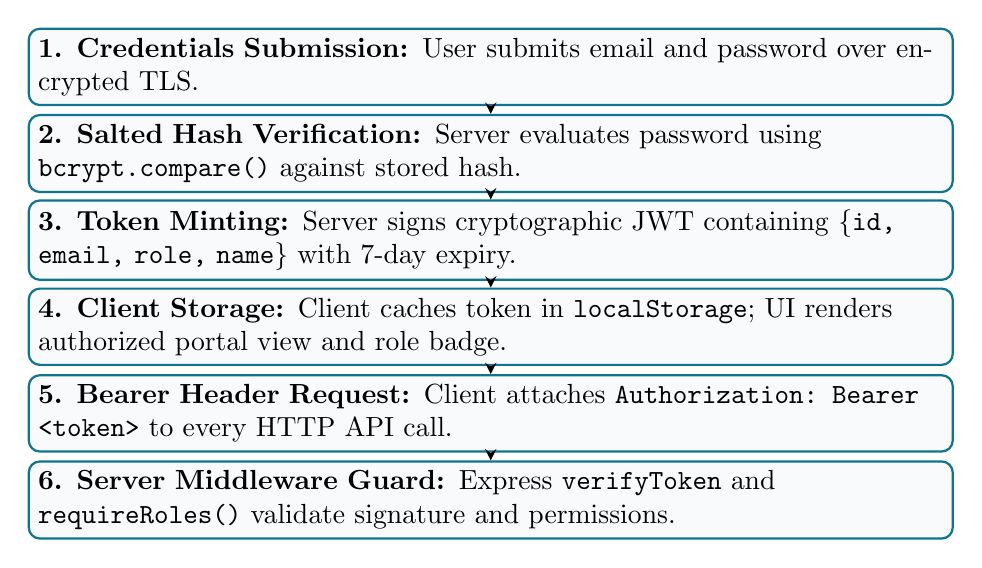
\begin{tikzpicture}[node distance=1.1cm, auto,
    block/.style={rectangle, draw=primary, fill=lightgray, thick, rounded corners, text width=11.5cm, minimum height=0.6cm, align=left},
    arrow/.style={thick, ->, >=stealth}]
    
    \node [block] (step1) {\textbf{1. Credentials Submission:} User submits email and password over encrypted TLS.};
    \node [block, below of=step1] (step2) {\textbf{2. Salted Hash Verification:} Server evaluates password using \texttt{bcrypt.compare()} against stored hash.};
    \node [block, below of=step2] (step3) {\textbf{3. Token Minting:} Server signs cryptographic JWT containing \texttt{\{id, email, role, name\}} with 7-day expiry.};
    \node [block, below of=step3] (step4) {\textbf{4. Client Storage:} Client caches token in \texttt{localStorage}; UI renders authorized portal view and role badge.};
    \node [block, below of=step4] (step5) {\textbf{5. Bearer Header Request:} Client attaches \texttt{Authorization: Bearer <token>} to every HTTP API call.};
    \node [block, below of=step5] (step6) {\textbf{6. Server Middleware Guard:} Express \texttt{verifyToken} and \texttt{requireRoles()} validate signature and permissions.};

    \draw [arrow] (step1) -- (step2);
    \draw [arrow] (step2) -- (step3);
    \draw [arrow] (step3) -- (step4);
    \draw [arrow] (step4) -- (step5);
    \draw [arrow] (step5) -- (step6);
\end{tikzpicture}
\caption{Cryptographic JWT Authentication and Middleware Guard Lifecycle}
\end{figure}

\subsection{6.2 Six-Tier Role-Based Privilege Matrix}
\begin{table}[H]
\centering
\footnotesize
\begin{tabularx}{\textwidth}{l p{3.2cm} X}
\toprule
\textbf{Role Identifier} & \textbf{Designation} & \textbf{System Permissions \& Scope} \\
\midrule
\texttt{superadmin} / \texttt{admin} & \textbf{Super Administrator} & Unrestricted full platform control: staff account provisioning, role modification, database maintenance, financial ledger audits, and emergency alert broadcasts. \\
\addlinespace
\texttt{manager} & \textbf{Operations Manager} & Management of Destination Catalog (DMS), flight schedules, accommodation inventory, vehicle fleet, and customer booking approvals. \\
\addlinespace
\texttt{accountant} & \textbf{Senior Accountant} & Real-time financial transaction ledger (Stripe, PayPal, bKash), payment verification, voucher receipts, and corporate B2B tax audits. \\
\addlinespace
\texttt{support} & \textbf{Support Specialist} & Customer leads inbox, traveler support ticketing, visa application clearance, and real-time passport status tracking. \\
\addlinespace
\texttt{moderator} & \textbf{Content Moderator} & Traveler review moderation (approvals/filtering), travel blog curation, and community travelogue publishing. \\
\addlinespace
\texttt{customer} & \textbf{Registered Traveler} & Public browsing, Custom Trip Builder, package checkout, personal wishlist, booking history (\texttt{/my-trips}), and review submission. \\
\bottomrule
\end{tabularx}
\caption{Enterprise Role-Based Access Control (RBAC) Hierarchy}
\end{table}

\newpage

% ==============================================================================
% SECTION 7: DATABASE DESIGN & E-R MODEL
% ==============================================================================
\section{Database Design \& Conceptual E-R Model}

\subsection{7.1 Conceptual Entity-Relationship (E-R) Diagram}
\begin{figure}[H]
\centering
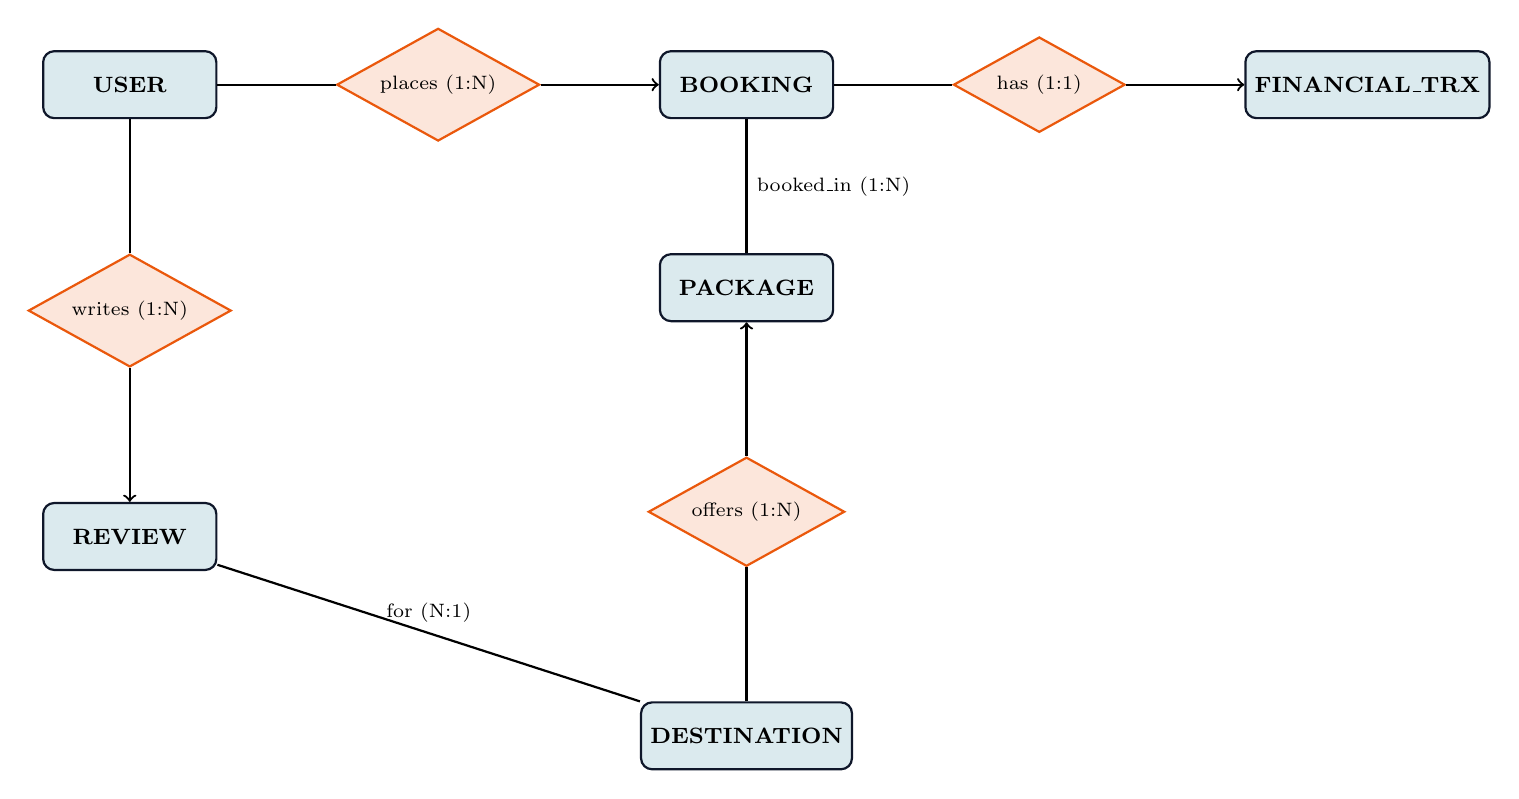
\begin{tikzpicture}[node distance=1.7cm and 1.5cm, auto,
    entity/.style={rectangle, draw=secondary, fill=primary!15, thick, rounded corners, minimum width=2.2cm, minimum height=0.85cm, font=\bfseries\footnotesize},
    rel/.style={diamond, draw=accent, fill=accent!15, thick, aspect=1.8, minimum width=1.9cm, font=\scriptsize}]

    % Nodes
    \node[entity] (user) {USER};
    \node[rel, right=of user] (places) {places (1:N)};
    \node[entity, right=of places] (booking) {BOOKING};
    
    \node[rel, below=of user] (writes) {writes (1:N)};
    \node[entity, below=of writes] (review) {REVIEW};
    
    \node[rel, right=of booking] (has) {has (1:1)};
    \node[entity, right=of has] (payment) {FINANCIAL\_TRX};

    \node[entity, below=of booking] (package) {PACKAGE};
    \node[rel, below=of package] (offers) {offers (1:N)};
    \node[entity, below=of offers] (destination) {DESTINATION};

    % Connections
    \draw[thick] (user) -- (places);
    \draw[thick, ->] (places) -- (booking);
    
    \draw[thick] (booking) -- (has);
    \draw[thick, ->] (has) -- (payment);

    \draw[thick] (package) -- node[right]{\scriptsize booked\_in (1:N)} (booking);
    \draw[thick] (destination) -- (offers);
    \draw[thick, ->] (offers) -- (package);

    \draw[thick] (user) -- (writes);
    \draw[thick, ->] (writes) -- (review);
    \draw[thick] (review) -- node[above]{\scriptsize for (N:1)} (destination);

\end{tikzpicture}
\caption{Conceptual Entity-Relationship (E-R) Diagram for TravelUp Global}
\end{figure}

\subsection{7.2 Relational Data Dictionary}
\begin{table}[H]
\centering
\scriptsize
\begin{tabularx}{\textwidth}{l l l X}
\toprule
\textbf{Table Name} & \textbf{Primary Key} & \textbf{Foreign Keys} & \textbf{Key Attributes \& System Purpose} \\
\midrule
\texttt{users} & \texttt{id} & None & \texttt{name, email, password, role, status, phone, preferred\_lang, avatar\_url} \\
\addlinespace
\texttt{destinations} & \texttt{id} & None & \texttt{name\_en, name\_bn, country, category, price\_usd, price\_bdt, rating, latitude, longitude} \\
\addlinespace
\texttt{packages} & \texttt{id} & \texttt{destination\_id} & \texttt{title\_en, title\_bn, duration\_days, price\_usd, price\_bdt, included\_services} \\
\addlinespace
\texttt{flights} & \texttt{id} & None & \texttt{flight\_code, airline, origin, destination, departure\_time, price\_usd, status} \\
\addlinespace
\texttt{hotels} & \texttt{id} & \texttt{destination\_id} & \texttt{name, star\_rating, city, address, base\_price, has\_elevator, is\_accessible} \\
\addlinespace
\texttt{transportation}& \texttt{id} & \texttt{destination\_id} & \texttt{title, vehicle\_type, service\_type, capacity, base\_price, status} \\
\addlinespace
\texttt{restaurants} & \texttt{id} & \texttt{destination\_id} & \texttt{name, cuisine\_type, is\_halal, is\_pure\_veg, price\_tier, address} \\
\addlinespace
\texttt{visa\_applications} & \texttt{id} & \texttt{user\_id} & \texttt{application\_no, traveler\_name, passport\_number, country, status} \\
\addlinespace
\texttt{bookings} & \texttt{id} & \texttt{user\_id} & \texttt{booking\_ref, customer\_name, package\_id, travel\_date, total\_price, status} \\
\addlinespace
\texttt{financial\_transactions} & \texttt{id} & \texttt{booking\_id} & \texttt{trx\_id, booking\_ref, gateway, currency, amount, status, date} \\
\addlinespace
\texttt{split\_payments} & \texttt{id} & \texttt{booking\_id} & \texttt{split\_token, student\_name, amount, payment\_status, trx\_timestamp} \\
\addlinespace
\texttt{travel\_alerts} & \texttt{id} & \texttt{destination\_id} & \texttt{title\_en, title\_bn, severity, message\_en, message\_bn, is\_active} \\
\bottomrule
\end{tabularx}
\caption{Production Relational Database Schema Specifications}
\end{table}

\newpage

% ==============================================================================
% SECTION 8: IMPLEMENTATION TIMELINE, FUTURE RESEARCH & CONCLUSION
% ==============================================================================
\section{Implementation Timeline, Future Research \& Conclusion}

\subsection{8.1 Execution Roadmap \& Milestone Schedule}
\begin{table}[H]
\centering
\scriptsize
\begin{tabularx}{\textwidth}{l p{3.8cm} X}
\toprule
\textbf{Phase / Milestone} & \textbf{Focus Area} & \textbf{Key Technical Deliverables} \\
\midrule
\textbf{Phase 1: Foundation} & Semantic Markup \& Layout & Semantic HTML5 structures, responsive CSS3 Flexbox/Grid layouts, Overleaf signoff. \\
\textbf{Phase 2: Persistence} & Relational Database & Hostinger MySQL schema initialization, Express.js REST API endpoints, connection pooling. \\
\textbf{Phase 3: Security} & Enterprise 6-Tier RBAC & JWT bearer issuance, password salting with \texttt{bcryptjs}, isolated portal route guards. \\
\textbf{Phase 4: Operations} & Master Services \& DMS & Destination Management System (DMS), IATA flight tables, hotels, ground fleet, visa tracker. \\
\textbf{Phase 5: Logistics} & Dynamic Trip Builder & Custom Trip Builder with live price calculation, \texttt{Skip Transport}, split-bill webhooks. \\
\textbf{Phase 6: Verification} & Edge-Case Testing & Validating 12 real-world travel scenarios, micro-interactions, floating toast notifications. \\
\textbf{Phase 7: Advanced} & Future Research Scale & WebXR 3D virtual tours, PWA offline sync, GDS telematics, and blockchain smart contracts. \\
\bottomrule
\end{tabularx}
\caption{Project Execution Roadmap and Milestone Schedule}
\end{table}

\subsection{8.2 Future Scope \& Innovative Research Roadmap}
\begin{itemize}[leftmargin=*]
    \item \textbf{Real-Time Flight Radar \& GDS Integration:} Integration with Amadeus/Sabre GDS APIs via WebSockets for live radar telematics, gate change notifications, and automated flight delay compensation processing.
    \item \textbf{WebXR 3D Virtual Tours:} Browser-native WebXR Device API and Three.js spatial panoramas, allowing travelers to inspect hotel room dimensions and heritage landmarks in 3D without external applications.
    \item \textbf{Blockchain Smart Contracts for Group Escrow:} Decentralized Polygon/Ethereum smart contracts for trustless group payments, releasing vendor funds upon tour quorum fulfillment and auto-refunding if minimum targets fail.
    \item \textbf{Predictive ML Fare Forecasting:} LSTM neural networks predicting airfare surges to advise ``Book Now vs. Wait'' accompanied by automated 48-hour price freeze locks.
\end{itemize}

\subsection{8.3 Academic Conclusion}
\textbf{TravelUp Global} decisively proves that modern travel discovery, itinerary compilation, and operational logistics cannot be conducted through primitive social media pages or manual chat conversations. By satisfying every benchmark of the \textbf{Markup \& Scripting Languages Lab} curriculum---semantic HTML5, hardware-accelerated CSS3, asynchronous client DOM scripting, Node.js REST services, relational MySQL persistence, and cryptographic JWT authorization---the platform achieves an exemplary standard of computer science rigor. It directly bridges the gap between theoretical web engineering and real-world commercial software scalability.

\end{document}
